% ============================================================================
% Scaling Curve: Data Size vs. Downstream Fine-tuning Performance
% Qwen2.5-1.5B + LoRA evaluated at 100, 522, 9478 training dialogues
% ============================================================================

\begin{figure}[t]
\centering
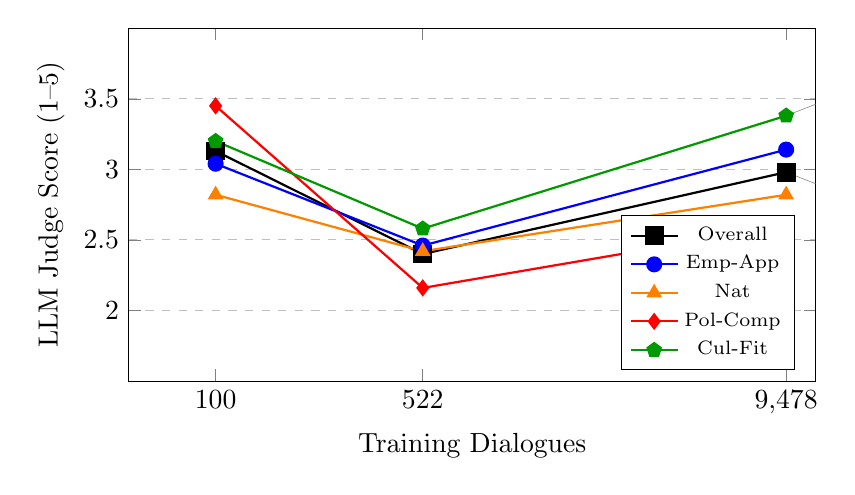
\begin{tikzpicture}
\begin{axis}[
    width=0.85\textwidth,
    height=0.5\textwidth,
    xlabel={Training Dialogues},
    ylabel={LLM Judge Score (1--5)},
    xmin=50, xmax=12000,
    xmode=log,
    log basis x=10,
    xtick={100, 522, 9478},
    xticklabels={100, 522, 9{,}478},
    ymin=1.5, ymax=4.0,
    ytick={2.0, 2.5, 3.0, 3.5},
    legend pos=south east,
    ymajorgrids=true,
    grid style=dashed,
    legend style={font=\scriptsize},
]

% Overall score
\addplot[color=black, mark=square*, thick, mark size=3pt]
coordinates {
(100, 3.13)
(522, 2.40)
(9478, 2.98)
};

% Emp-App
\addplot[color=blue, mark=*, thick, mark size=2.5pt]
coordinates {
(100, 3.04)
(522, 2.46)
(9478, 3.14)
};

% Nat
\addplot[color=orange, mark=triangle*, thick, mark size=2.5pt]
coordinates {
(100, 2.82)
(522, 2.42)
(9478, 2.82)
};

% Pol-Comp
\addplot[color=red, mark=diamond*, thick, mark size=2.5pt]
coordinates {
(100, 3.45)
(522, 2.16)
(9478, 2.60)
};

% Cul-Fit
\addplot[color=green!60!black, mark=pentagon*, thick, mark size=2.5pt]
coordinates {
(100, 3.20)
(522, 2.58)
(9478, 3.38)
};

\legend{Overall, Emp-App, Nat, Pol-Comp, Cul-Fit}

% Annotation for 522->9478 gain
\node[coordinate, pin={[font=\scriptsize]above right:{+31.0\% Cul-Fit}}]
  at (axis cs:9478, 3.38) {};

% Annotation for overall recovery
\node[coordinate, pin={[font=\scriptsize]below right:{+24.2\% Overall}}]
  at (axis cs:9478, 2.98) {};

\end{axis}
\end{tikzpicture}
\caption{Downstream fine-tuning scaling: Qwen2.5-1.5B + LoRA trained on 100, 522, and 9{,}478 dialogues. The full dataset (9{,}478) consistently outperforms the 522-dialogue subset, with Cultural-Fit showing the strongest scaling benefit (+31.0\%). The 100-dialogue baseline achieves competitive scores through safe, generic responses.}
\label{fig:scaling_curve}
\end{figure}
